% Provenance (never printed): cycle 4 SVT, "La planete Terre": the dynamics of
% the Earth's outer shell, plates and their boundaries, continental drift as a
% history of ideas; see sources/outline_sources.md. Pilot chapter, 2026-10-22.
\chapter{板块构造：移动的拼图}\label{ch:g7:plate-tectonics}

在桌上摊开一张\omterm{def:g3:continents-and-oceans:world-map}{世界地图}，看看大西洋两岸。巴西隆起的\omterm{def:g1:landscapes-around-us:water}{海岸}，
仿佛正好能嵌入非洲西\omterm{def:g1:landscapes-around-us:water}{海岸}的凹处，
就像有人把一整块陆地切成两半，
再把两半推开。最早绘出两岸清晰\omterm{def:g2:drawing-to-map:map}{地图}的人，
立刻注意到了这一点。三个世纪里，它一直只是一个奇闻。
二十世纪，它成为一种理论的出发点，这一理论如今能够解释，
为什么日本地面会震动，为什么安第斯\omterm{def:g4:world-physical-map:range}{山脉}如此高耸，
为什么冰岛正在缓慢变宽——以及为什么桌上这张\omterm{def:g2:drawing-to-map:map}{地图}
只是一个正在移动的世界的一张快照。

\begin{omfigure}

\includegraphics[width=0.62\linewidth]{images/book1/ai/g7-puzzle-map.jpg}

{\small 南美洲紧邻非洲：拼图上，贴合只是一个游戏；
在真实的地球上，它却是一条线索。}
\end{omfigure}

\begin{recall}
地球有三个主要圈层：薄而坚硬的\emph{\omterm{def:g6:inside-the-earth:layers}{地壳}}，
厚厚的热\omterm{def:g3:stones-pebbles-sand:rock}{岩石}构成的\emph{\omterm{def:g6:inside-the-earth:layers}{地幔}}，以及金属质的\emph{\omterm{def:g6:inside-the-earth:layers}{地核}}；温度随深度增加而升高
（见\cref{ch:g6:inside-the-earth}）。\omterm{def:g3:continents-and-oceans:globe}{地球仪}上某地的位置，
由它的\omterm{def:g6:latitude-longitude:latitude}{纬度}和\omterm{def:g6:latitude-longitude:longitude}{经度}确定（见\cref{ch:g6:latitude-longitude}）。
\end{recall}

\section{曾经相互拼合的大陆}

\begin{definition}[大陆漂移]\label{def:g7:plate-tectonics:continental-drift}
\emph{大陆漂移}\index{大陆漂移}是指：\omterm{def:g3:continents-and-oceans:continent}{大陆}
在地球表面上缓慢地移动，
因此它们的位置，以及它们之间\omterm{def:g2:water-on-earth:ocean}{海洋}的形状，
在漫长的岁月中已经发生了变化。
\end{definition}

\begin{definition}[超大陆]\label{def:g7:plate-tectonics:supercontinent}
\emph{超大陆}\index{超大陆}是指一个单一的陆块，
由全部或几乎全部\omterm{def:g3:continents-and-oceans:continent}{大陆}连接在一起而形成。最后一个超\omterm{def:g3:continents-and-oceans:continent}{大陆}，
\emph{泛大陆}\index{泛大陆}（希腊语意为“所有陆地”）
约在 2.25 亿至 2 亿年前开始解体。
% ledger: usgs:pangaea-breakup
\end{definition}

第一位以证据为支撑、把\omterm{def:g7:plate-tectonics:continental-drift}{大陆漂移}当作真实理论加以捍卫的科学家，
是魏格纳。他收集了四类线索。

\begin{enumerate}
  \item \textbf{\omterm{def:g1:landscapes-around-us:water}{海岸}的形状。}南美洲与非洲如同拼图的两块，
        严丝合缝，
        其他几处\omterm{def:g1:landscapes-around-us:water}{海岸}线也是如此。
  \item \textbf{化石。}同样的古代动物和植物化石，出现在
        如今被数千千米\omterm{def:g2:water-on-earth:ocean}{海洋}隔开的\omterm{def:g3:continents-and-oceans:continent}{大陆}上。
        \emph{Mesosaurus}是一种生活在\omterm{def:g2:water-on-earth:salt-fresh}{淡水}中的小型爬行动物，
        它不可能游过大洋，
        但它的化石同时出现在巴西和非洲南部。
  \item \textbf{\omterm{def:g3:stones-pebbles-sand:rock}{岩石}。}相同种类、相同年代的\omterm{def:g3:stones-pebbles-sand:rock}{岩石}，以及形状相同的古老\omterm{def:g4:world-physical-map:range}{山脉}，
        在一岸中断，
        又在对岸接续，正如撕碎的报纸上的文字行。
  \item \textbf{古\omterm{def:g5:weather-and-climate:climate}{气候}。}煤是由温暖沼泽森林中的植物形成的，
        这种煤见于\omterm{def:g3:continents-and-oceans:poles}{南极}洲；
        古冰川留下的痕迹，见于如今炎热干燥的非洲部分地区。
        这些陆地过去一定处于其他\omterm{def:g5:weather-and-climate:climate-zone}{气候带}，
        位于其他\omterm{def:g6:latitude-longitude:latitude}{纬度}。
\end{enumerate}
% ledger: usgs:coal-antarctica, usgs:fossil-map

\begin{omfigure}
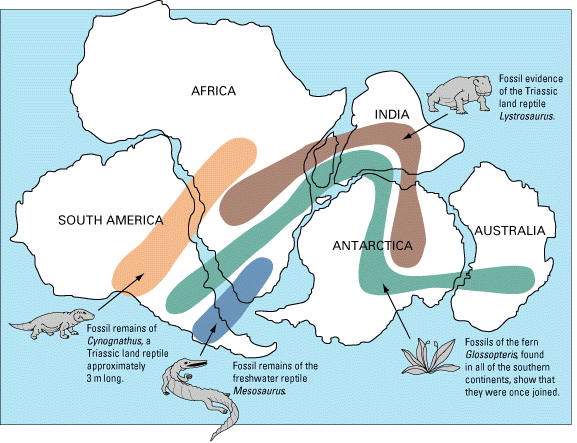
\includegraphics[width=0.86\linewidth]{images/book1/g7-usgs-fossil-map.png}

{\small 将南方\omterm{def:g3:continents-and-oceans:continent}{大陆}拼回原位。每条有色带连接着如今发现同一化石物种的地点：
陆生爬行动物\emph{Cynognathus}和\emph{Lystrosaurus}、\omterm{def:g2:water-on-earth:salt-fresh}{淡水}爬行动物
\emph{Mesosaurus}以及蕨类植物\emph{Glossopteris}。\omterm{def:g3:continents-and-oceans:continent}{大陆}分开时，色带四散；
拼合之后，色带便连成一片，不再中断。
\omterm{def:g2:drawing-to-map:map}{地图}来源：美国地质调查局，
\emph{This Dynamic Earth}（公有领域）。}
\end{omfigure}

\begin{history}[魏格纳的设想，1912--1930]
% ledger: usgs:wegener-1912, usgs:wegener-death, usgs:jeffreys
魏格纳，一位 32 岁的德国气象学家，于 1912 年在两篇文章中提出了\omterm{def:g7:plate-tectonics:continental-drift}{大陆漂移}理论。
多数地质学家拒绝接受这一理论。
最有力的反对意见是：魏格纳无法说明\emph{什么}使\omterm{def:g3:continents-and-oceans:continent}{大陆}移动。
他设想\omterm{def:g3:continents-and-oceans:continent}{大陆}是穿过洋底\omterm{def:g3:stones-pebbles-sand:rock}{岩石}而前行的；
物理学家哈罗德·杰弗里斯证明，坚硬的\omterm{def:g3:continents-and-oceans:continent}{大陆}不可能这样移动而不破碎。
魏格纳继续收集证据，
1930 年，他在一次考察途中于格陵兰冰盖上去世。
他所缺少的答案，来自 1950 年代以后对洋底的探测：
这一内容将在以后的年级中讲述。
\end{history}

\section{板块}

魏格纳的线索是对的，但他选错了拼图的块。
移动的不仅是\omterm{def:g3:continents-and-oceans:continent}{大陆}：地球的整个外壳，
无论在\omterm{def:g3:continents-and-oceans:continent}{大陆}之下还是在\omterm{def:g2:water-on-earth:ocean}{海洋}之下，都被分割成了许多块。

\begin{definition}[构造板块]\label{def:g7:plate-tectonics:plate}
\emph{构造板块}\index{构造板块}（或简称板块）是
构成地球外壳一部分的大块坚硬\omterm{def:g3:stones-pebbles-sand:rock}{岩石}。板块
由\omterm{def:g6:inside-the-earth:layers}{地壳}以及\omterm{def:g6:inside-the-earth:layers}{地幔}最上部寒冷而坚硬的部分组成，
平均厚度至少为 80 千米；
它在其下方更热、更软的\omterm{def:g6:inside-the-earth:layers}{地幔}之上缓慢移动。
% ledger: usgs:lithosphere-80km
\end{definition}

\begin{definition}[板块构造]\label{def:g7:plate-tectonics:plate-tectonics}
\emph{板块构造}\index{板块构造}是这样一种理论：地球外壳
被划分为若干板块，这些板块彼此相对移动，
并且大多数\omterm{def:g4:volcanoes-earthquakes-first-look:earthquake}{地震}、\omterm{def:g4:volcanoes-earthquakes-first-look:volcano}{火山}和\omterm{def:g4:world-physical-map:range}{山脉}
都产生于板块相遇的地方。
\end{definition}

\begin{remark}[板块有多少个？]\label{rem:g7:plate-tectonics:how-many}
% ledger: usgs:plates-dozen, pb2002:count
约有十几个板块较大，许多板块则很小。地质学家
使用的一幅详细\omterm{def:g2:drawing-to-map:map}{地图}标出了其中 52 个。一个板块可以承载一块\omterm{def:g3:continents-and-oceans:continent}{大陆}、一片\omterm{def:g2:water-on-earth:ocean}{海洋}，或
两者兼有：南美洲板块承载了整个南美洲以及
南大西洋的西半部。面积最大的太平洋板块，
几乎不承载任何陆地。
\end{remark}

\begin{omfigure}
\begin{tikzpicture}
\begin{axis}[ommap, width=\linewidth, xtick={-180,-90,...,180}, ytick={-60,0,60}]
\addplot[fill=omLithAlluv, draw=black!45, line width=0.2pt] table {figdata/out/shared-geo-land.dat};
\addplot[omRidge, line width=0.8pt] table {figdata/out/shared-geo-school-ridge.dat};
\addplot[omRidge!70!black, line width=0.8pt] table {figdata/out/shared-geo-school-transform.dat};
\addplot[omTrench, line width=0.8pt] table {figdata/out/shared-geo-school-subduction.dat};
\addplot[fill=omTrench, draw=none] table {figdata/out/shared-geo-school-teeth.dat};
\addplot[black!65, line width=0.8pt] table {figdata/out/shared-geo-school-collision.dat};
\begin{scope}[every node/.style={font=\scriptsize\bfseries, text=black!85,
    fill=white, fill opacity=0.75, text opacity=1, inner sep=1pt, align=center}]
  \node at (axis cs:-150,12) {太平洋板块};
  \node at (axis cs:-103,52) {北美 \\板块};
  \node at (axis cs:-48,-12) {南美 \\板块};
  \node at (axis cs:85,57) {欧亚 \\板块};
  \node at (axis cs:18,8) {非洲 \\板块};
  \node at (axis cs:10,-75) {南极 \\板块};
  \node at (axis cs:78,11) {印度 \\板块};
  \node at (axis cs:128,-26) {澳大利亚 \\板块};
  \node at (axis cs:-95,-22) {纳斯卡 \\板块};
  \node at (axis cs:50,20) {阿拉伯 \\板块};
\end{scope}
\end{axis}
\end{tikzpicture}

{\small 主要\omterm{def:g7:plate-tectonics:plate}{构造板块}。红色：板块相互远离；蓝色带三角形：一个板块俯冲到另一个板块之下
（三角形位于保持在上方的板块一侧）；
灰色：板块挤压在一起，形成宽广的\omterm{def:g4:world-physical-map:range}{山脉}带；
深红色：板块彼此错动滑过。边界据
P.~Bird（2003）；\omterm{def:g1:landscapes-around-us:water}{海岸}线取自 Natural Earth。}
\end{omfigure}

如何判断一个板块在哪里结束、下一个板块从哪里开始？
看看地球哪里最不安分。

\begin{proposition}[地震与火山勾勒出板块边界]\label{prop:g7:plate-tectonics:restless}
% ledger: data:usgs-comcat, data:pb2002 (share computed in figdata/grade-7/quakes_on_boundaries.py)
\omterm{def:g4:volcanoes-earthquakes-first-look:earthquake}{地震}和\omterm{def:g4:volcanoes-earthquakes-first-look:volcano}{火山}并非随机散布在地球上：它们大多
沿狭长的带状区域分布，这些带正是板块的边缘。
在 1976 年至 2025 年间记录到的 7\,031 次震级为 6 级或以上的\omterm{def:g4:volcanoes-earthquakes-first-look:earthquake}{地震}中，
有 6\,472 次——即 92\,\%——发生在距离\omterm{def:g7:plate-tectonics:plate-boundary}{板块边界}
不足 \qty{300}{km} 的地方。
\end{proposition}

\begin{omfigure}
\begin{tikzpicture}
\begin{axis}[ommap, width=\linewidth, xtick={-180,-90,...,180}, ytick={-60,0,60},
  legend style={at={(0.02,0.04)}, anchor=south west, font=\scriptsize,
  fill=white, fill opacity=0.85, text opacity=1, draw=black!40}]
\addplot[fill=omLithAlluv, draw=black!45, line width=0.2pt, forget plot] table {figdata/out/shared-geo-land.dat};
\addplot[only marks, mark=*, mark size=0.45pt, omThm!85!black] table[x=lon, y=lat] {figdata/out/grade-7-quakes_on_boundaries-map.dat};
\addlegendentry{地震，震级 6.5 或以上，1976--2025}
\addplot[only marks, mark=triangle*, mark size=1.1pt, black] table {figdata/out/shared-geo-volcanoes.dat};
\addlegendentry{近 12\,000 年内活动的火山}
\end{axis}
\end{tikzpicture}

{\small 大\omterm{def:g4:volcanoes-earthquakes-first-look:earthquake}{地震}与近期\omterm{def:g4:volcanoes-earthquakes-first-look:volcano}{火山}。对照上方的板块图，
圆点与三角形勾勒出了\omterm{def:g7:plate-tectonics:plate-boundary}{板块边界}。数据来源：美国地质调查局
\omterm{def:g4:volcanoes-earthquakes-first-look:earthquake}{地震}目录；史密森学会全球\omterm{def:g4:volcanoes-earthquakes-first-look:volcano}{火山}活动
计划。}
\end{omfigure}

\section{三类板块边界}

\begin{definition}[板块边界]\label{def:g7:plate-tectonics:plate-boundary}
\emph{板块边界}\index{板块边界}是两个板块相遇的线，或
狭窄的区域。根据两个板块彼此相对运动的方式，
边界可分为以下三类：
\begin{itemize}
  \item 在\emph{离散型边界}\index{离散型边界}处，两个板块
        相互远离；
  \item 在\emph{汇聚型边界}\index{汇聚型边界}处，两个板块
        相互靠近；
  \item 在\emph{转换型边界}\index{转换型边界}处，两个板块彼此错动，
        并排滑过。
\end{itemize}
\end{definition}

\begin{example}[离散型边界：冰岛与东非]\label{ex:g7:plate-tectonics:divergent}
% ledger: usgs:iceland, usgs:east-africa
大西洋中部延伸着一条海底\omterm{def:g4:world-physical-map:range}{山脉}链，
即大西洋中脊，其两侧的板块相互远离。
来自\omterm{def:g6:inside-the-earth:layers}{地幔}的热\omterm{def:g3:stones-pebbles-sand:rock}{岩石}涌入裂隙，部分熔化，
形成新的海底：\omterm{def:g7:plate-tectonics:plate-boundary}{离散型边界}不断生成新的板块。
冰岛是这条山脊露出海面的一段：那里北美板块向西移动，
欧亚板块向东移动，岛屿正被缓慢撕裂。1975 年至 1984 年间，
岛北部克拉夫拉\omterm{def:g4:volcanoes-earthquakes-first-look:volcano}{火山}附近的裂缝总共扩宽了约 7 米。
\omterm{def:g7:plate-tectonics:plate-boundary}{离散型边界}也可以切穿\omterm{def:g3:continents-and-oceans:continent}{大陆}：沿东非裂谷，
非洲正在开裂，
而红海是一个年轻的大洋，
它已将阿拉伯半岛与非洲分开。
\end{example}

\begin{example}[汇聚型边界：安第斯山脉与喜马拉雅山脉]\label{ex:g7:plate-tectonics:convergent}
% ledger: usgs:trench-depth, usgs:himalaya
在南美洲西\omterm{def:g1:landscapes-around-us:water}{海岸}外，纳斯卡板块承载着\omterm{def:g2:water-on-earth:ocean}{海洋}，向南美板块移动，
南美板块承载着\omterm{def:g3:continents-and-oceans:continent}{大陆}。较重的大洋板块弯曲，
并俯冲到\omterm{def:g3:continents-and-oceans:continent}{大陆}之下，深入\omterm{def:g6:inside-the-earth:layers}{地幔}。
在它下沉的线上，海底陷入深深的海沟；
在俯冲板块上方，陆地频繁发生\omterm{def:g4:volcanoes-earthquakes-first-look:earthquake}{地震}，
并布满\omterm{def:g4:volcanoes-earthquakes-first-look:volcano}{火山}：这就是安第斯\omterm{def:g4:world-physical-map:range}{山脉}。在西太平洋，一个大洋板块俯冲到另一个之下，
海沟是地球上最深的地方：
马里亚纳海沟的深度接近 \qty{11000}{m}。当两个\omterm{def:g3:continents-and-oceans:continent}{大陆}相遇时，
两者都不会下沉：\omterm{def:g6:inside-the-earth:layers}{地壳}发生褶皱并增厚。约 5000 万年前印度与亚洲相撞，
两个板块至今仍在挤压，
喜马拉雅\omterm{def:g4:world-physical-map:range}{山脉}和青藏高原正是由此隆起的。
\end{example}

\begin{example}[转换型边界：圣安德烈亚斯断层]\label{ex:g7:plate-tectonics:transform}
% ledger: usgs:san-andreas, usgs:san-andreas-photo
在加利福尼亚，太平洋板块沿圣安德烈亚斯断层
向西北方向滑过北美板块，断层全长约 \qty{1300}{km}。
那里既没有板块生成，也没有板块消亡；两个板块
相互摩擦着错动，这种摩擦引发的震动就是\omterm{def:g4:volcanoes-earthquakes-first-look:earthquake}{地震}。
\end{example}

\begin{omfigure}
\begin{tikzpicture}[x=1cm, y=1cm, font=\small]
  % mantle
  \fill[omLithGranite!45] (0,-3.3) rectangle (12.4,-0.85);
  \node[font=\footnotesize, text=black!75] at (2.6,-2.6) {地幔：炽热而柔软};
  % sea water
  \fill[omSea] (0,0) -- (0,-0.75) -- (1.5,-0.6) -- (3,-0.25) -- (4.5,-0.6)
    -- (7.4,-0.8) -- (8.0,-1.2) -- (8.6,-0.6) -- (8.9,0) -- cycle;
  % oceanic plates (the ridge at x = 3, the trench at x = 8)
  \fill[omLithBasalt!70] (0,-0.75) -- (1.5,-0.6) -- (3,-0.25) -- (4.5,-0.6)
    -- (7.4,-0.8) -- (8.0,-1.2) -- (9.6,-2.3) -- (10.2,-3.3) -- (9.5,-3.3)
    -- (8.6,-2.2) -- (7.5,-1.55) -- (4.5,-1.35) -- (3.2,-0.95) -- (2.8,-0.95)
    -- (1.5,-1.35) -- (0,-1.45) -- cycle;
  % continental plate
  \fill[omLithSand!80] (8.6,-0.6) -- (8.9,0) -- (9.4,0.35) -- (9.8,0.9)
    -- (10.2,0.35) -- (12.4,0.2) -- (12.4,-1.9) -- (10.6,-1.9) -- (9.6,-2.3)
    -- (8.0,-1.2) -- cycle;
  \draw[black!70, line width=0.5pt] (0,-0.75) -- (1.5,-0.6) -- (3,-0.25)
    -- (4.5,-0.6) -- (7.4,-0.8) -- (8.0,-1.2) -- (8.6,-0.6) -- (8.9,0)
    -- (9.4,0.35) -- (9.8,0.9) -- (10.2,0.35) -- (12.4,0.2);
  \draw[black!45, densely dashed] (0,0) -- (8.9,0);
  % magma: under the ridge and under the volcano
  \fill[omThm!80] (2.85,-0.95) -- (3,-0.3) -- (3.15,-0.95) -- cycle;
  \draw[omThm!80, line width=1.4pt, -{Stealth[length=2.2mm]}] (3,-1.85) -- (3,-1.0);
  \draw[omThm!80, line width=1.2pt, decorate, decoration={snake, amplitude=0.6pt,
    segment length=4pt}] (9.8,-2.45) -- (9.8,0.75);
  % plate motions
  \draw[black, line width=1pt, -{Stealth[length=2.4mm]}] (2.5,-0.75) -- (1.3,-0.95);
  \draw[black, line width=1pt, -{Stealth[length=2.4mm]}] (3.5,-0.75) -- (5.4,-1.05);
  \draw[black, line width=1pt, -{Stealth[length=2.4mm]}] (12.1,-0.85) -- (10.9,-0.85);
  \draw[black, line width=1pt, -{Stealth[length=2.4mm]}] (8.7,-1.75) -- (9.3,-2.25);
  % labels
  \node[font=\footnotesize, align=center, above] at (3,0.05) {离散型边界：\\洋脊};
  \node[font=\footnotesize, align=center, below] at (6.9,-1.95) {汇聚型边界：\\大洋板块下沉};
  \draw[black!60, thin] (8.0,-1.25) -- (7.6,-1.9);
  \node[font=\footnotesize, above] at (8.0,0.05) {海沟};
  \draw[black!60, thin] (8.0,0.05) -- (8.0,-1.1);
  \node[font=\footnotesize, above] at (9.8,0.95) {火山};
  \node[font=\footnotesize] at (11.4,-0.4) {大陆};
  \node[font=\footnotesize] at (1.2,-1.6) {大洋板块};
  \node[font=\footnotesize, text=black!70] at (5.6,-0.32) {海洋};
\end{tikzpicture}

\medskip
\begin{tikzpicture}[font=\small]
  \fill[omLithBasalt!45] (0,0) rectangle (2.4,2.2);
  \fill[omLithSand!70] (2.4,0) rectangle (4.8,2.2);
  \draw[fault] (2.4,-0.1) -- (2.4,2.3);
  \draw[black, line width=1pt, -{Stealth[length=2.4mm]}] (1.2,0.5) -- (1.2,1.7);
  \draw[black, line width=1pt, -{Stealth[length=2.4mm]}] (3.6,1.7) -- (3.6,0.5);
  \node[font=\footnotesize, below] at (1.2,-0.1) {板块 A};
  \node[font=\footnotesize, below] at (3.6,-0.1) {板块 B};
  \node[font=\footnotesize, align=left, anchor=west] at (5.1,1.1)
    {转换型边界，俯视：\\两板块相互错动；\\没有板块生成或消亡};
\end{tikzpicture}

{\small 上图：穿过两个\omterm{def:g7:plate-tectonics:plate-boundary}{板块边界}的剖面（未按比例；深度被大幅夸大）。在洋脊处，
板块彼此分离，热\omterm{def:g3:stones-pebbles-sand:rock}{岩石}从\omterm{def:g6:inside-the-earth:layers}{地幔}上涌；在海沟处，大洋板块俯冲到\omterm{def:g3:continents-and-oceans:continent}{大陆}之下，
其上方熔融的\omterm{def:g3:stones-pebbles-sand:rock}{岩石}为\omterm{def:g4:volcanoes-earthquakes-first-look:volcano}{火山}提供岩浆。
下图：
从上方俯视的\omterm{def:g7:plate-tectonics:plate-boundary}{转换型边界}。}
\end{omfigure}

\begin{omfigure}
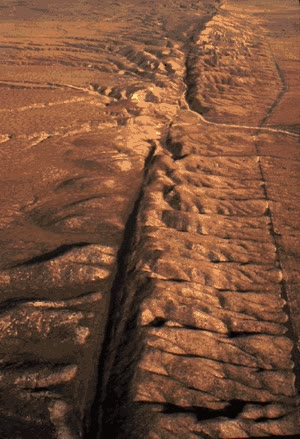
\includegraphics[width=0.28\linewidth]{images/book1/g7-usgs-san-andreas.jpg}

{\small 从飞机上看到的加利福尼亚卡里佐\omterm{def:g1:landscapes-around-us:landform}{平原}上的圣安德烈亚斯断层：
这条又长又直的\omterm{def:g1:landscapes-around-us:landform}{山谷}是太平洋板块（左）与北美板块（右）之间的边界。
照片：
Robert E. 华莱士, U.S. Geological Survey（公有领域）。}
\end{omfigure}

\begin{method}[识别板块边界]\label{met:g7:plate-tectonics:recognise}
要判断两个板块之间是哪一种边界：
\begin{enumerate}
  \item 在板块运动图上，找出边界两侧的
        箭头；
  \item 若箭头背离边界，则为离散型；若箭头指向边界，
        则为汇聚型；若箭头与边界平行且方向相反，
        则为转换型；
  \item 对照\omterm{def:g1:landscapes-around-us:landform}{地貌}检验：大洋中央的洋脊或横穿\omterm{def:g3:continents-and-oceans:continent}{大陆}的
        裂谷属于\omterm{def:g7:plate-tectonics:plate-boundary}{离散型边界}；深海沟与成排的\omterm{def:g4:volcanoes-earthquakes-first-look:volcano}{火山}，
        或高大的\omterm{def:g4:world-physical-map:range}{山脉}，属于\omterm{def:g7:plate-tectonics:plate-boundary}{汇聚型边界}；
        既无海沟也无\omterm{def:g4:world-physical-map:range}{山脉}、只有一条又长又直的断层的，
        属于\omterm{def:g7:plate-tectonics:plate-boundary}{转换型边界}。
\end{enumerate}
\end{method}

\section{板块移动有多快？}

\begin{proposition}[每年几厘米]\label{prop:g7:plate-tectonics:speed}
% ledger: data:pb2002 (speeds computed in figdata/grade-7/plate_speeds.py), usgs:mar-rate
两个相邻板块之间的相对运动速率约为
每年几厘米：从北大西洋的约每年 2 厘米，
到东太平洋海隆的每年超过 14 厘米，
后者是地球上扩张最快的洋脊。
\end{proposition}

\begin{omfigure}
\begin{tikzpicture}
\begin{axis}[xbar, width=0.82\linewidth, height=5.4cm, xmin=0, xmax=16.5,
  ytick={1,...,6}, yticklabels={北大西洋洋脊,南大西洋洋脊,
  圣安德烈亚斯断层,喜马拉雅山脉,秘鲁–智利海沟,东太平洋海隆},
  y tick label style={font=\small}, tick label style={font=\small},
  xlabel={一个板块相对另一个板块的速率（厘米每年）},
  label style={font=\small}, bar width=7pt, axis x line=bottom,
  axis y line=left, axis line style={-}, enlarge y limits=0.12,
  nodes near coords, nodes near coords style={font=\scriptsize},
  every node near coord/.append style={/pgf/number format/fixed,
  /pgf/number format/precision=1, /pgf/number format/fixed zerofill}]
\addplot[fill=omDef!55, draw=omDef!80!black] table[x=speed_cm_a, y=rank] {figdata/out/grade-7-plate_speeds.dat};
\end{axis}
\end{tikzpicture}

{\small 六条边界处板块的运动速率：沿各边界取平均值，
根据 P.~Bird 的板块模型（2003）计算。}
\end{omfigure}

\begin{method}[由厘米每年换算为千米每百万年]\label{met:g7:plate-tectonics:convert}
千米合 \num{100000} 厘米。速率为每年 \qty{1}{cm}，
若保持百万年，则走过 \num{1000000} 厘米，
即 \qty{10}{km}。由此可得：
\[
  1\ \text{厘米每年} = 10\ \text{千米每百万年}.
\]
将以厘米每年计的速率乘以 10，得到以千米每
百万年计的速率；再乘以百万年数，得到以千米计的距离，
或将距离除以速率，得到时间。
\end{method}

\begin{example}[大西洋在扩大]\label{ex:g7:plate-tectonics:atlantic}
% ledger: usgs:mar-rate
平均而言，大西洋中脊两侧以约
\qty{2.5}{cm} 每年的速率相互远离，即每百万年 \qty{25}{km}。
经过 1 亿年便是 \qty{2500}{km}：只要持续
足够久，一个在一生中难以察觉的慢速，便能张开一片\omterm{def:g2:water-on-earth:ocean}{海洋}。
\end{example}

\begin{remark}[今天如何测量运动]\label{rem:g7:plate-tectonics:gps}
% ledger: usgs:gps
如此缓慢的运动如今可以直接测量。固定在\omterm{def:g3:stones-pebbles-sand:rock}{基岩}上的
常驻站接收定位卫星的信号，并自行算出
自身位置，逐日测定，精度达到几毫米。
经过几年，位于不同板块上的观测站
被观测到相互远离或靠近，其速率与由\omterm{def:g3:stones-pebbles-sand:rock}{岩石}推算出的数百万年间的速率相当。
卫星定位本身在\cref{ch:g9:maps-of-the-earth}中讨论。
\end{remark}

\begin{omfigure}
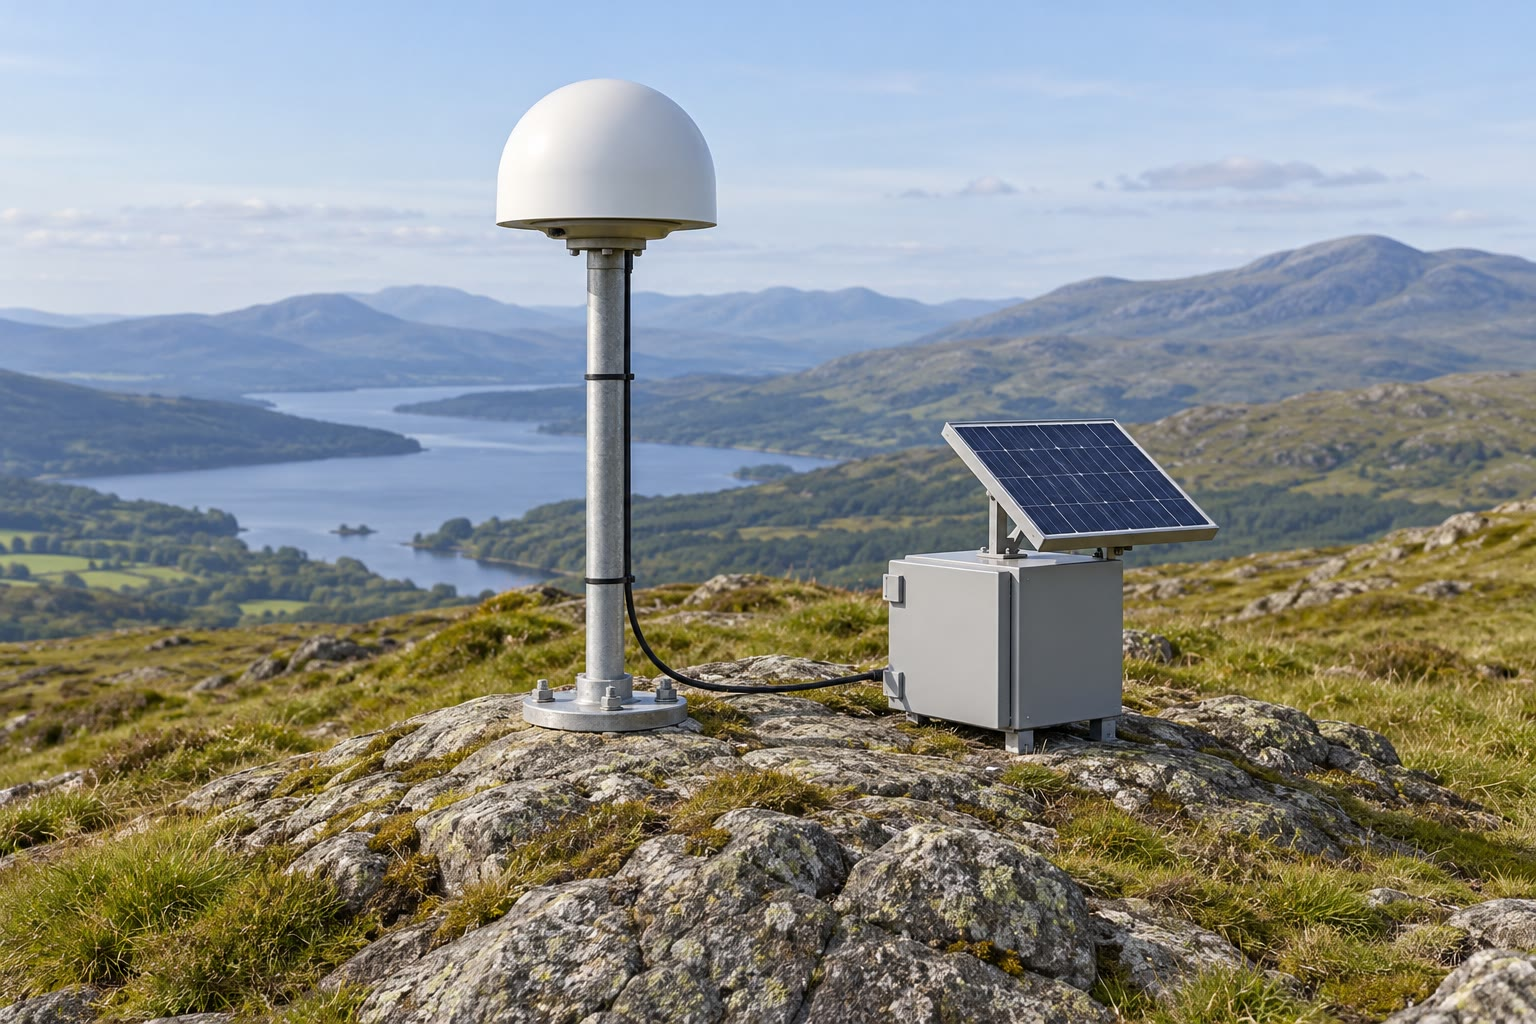
\includegraphics[width=0.55\linewidth]{images/book1/ai/g7-gps-station.jpg}

{\small 常驻定位站：其天线固定在
\omterm{def:g3:stones-pebbles-sand:rock}{岩石}上，因此随板块一同移动。}
\end{omfigure}

\section{练习}

\begin{exercise}[$\star$]\label{exo:g7:plate-tectonics:1}
什么是\omterm{def:g7:plate-tectonics:continental-drift}{大陆漂移}？给出魏格纳用来
支持该学说的四类证据。
\end{exercise}

\begin{exercise}[$\star$]\label{exo:g7:plate-tectonics:2}
说出三类\omterm{def:g7:plate-tectonics:plate-boundary}{板块边界}，并分别说明两侧板块
如何相对运动。
\end{exercise}

\begin{exercise}[$\star$]\label{exo:g7:plate-tectonics:3}
观察\omterm{def:g4:volcanoes-earthquakes-first-look:earthquake}{地震}与\omterm{def:g4:volcanoes-earthquakes-first-look:volcano}{火山}分布图。说出世界上大\omterm{def:g4:volcanoes-earthquakes-first-look:earthquake}{地震}
频发的两个地区，以及
内部几乎没有大\omterm{def:g4:volcanoes-earthquakes-first-look:earthquake}{地震}的一个\omterm{def:g3:continents-and-oceans:continent}{大陆}。
\end{exercise}

\begin{exercise}[$\star$]\label{exo:g7:plate-tectonics:4}
\emph{Mesosaurus}是一种生活在\omterm{def:g2:water-on-earth:salt-fresh}{淡水}中的小型爬行动物，其化石
见于巴西和非洲南部。这一现象为何能说明这两块
\omterm{def:g3:continents-and-oceans:continent}{大陆}曾经相连？
\end{exercise}

\begin{exercise}[$\star\star$]\label{exo:g7:plate-tectonics:5}
煤见于\omterm{def:g3:continents-and-oceans:poles}{南极}洲。这说明形成煤的
\omterm{def:g5:weather-and-climate:climate}{气候}条件如何，并能推断出当时\omterm{def:g3:continents-and-oceans:poles}{南极}洲
位于何处？
\end{exercise}

\begin{exercise}[$\star\star$]\label{exo:g7:plate-tectonics:6}
说出下列各处分别是哪一类边界：大西洋
中脊、安第斯\omterm{def:g4:world-physical-map:range}{山脉}、圣安德烈亚斯断层、喜马拉雅\omterm{def:g4:world-physical-map:range}{山脉}、东非
裂谷。
\end{exercise}

\begin{exercise}[$\star\star$]\label{exo:g7:plate-tectonics:7}
将速率 \qty{2.5}{cm} 每年换算为每百万年
多少千米。以此速率，边界两侧的两点
经过 6000 万年将相距多远？
\end{exercise}

\begin{exercise}[$\star\star$]\label{exo:g7:plate-tectonics:8}
1975 年至 1984 年——共九年——冰岛
克拉夫拉\omterm{def:g4:volcanoes-earthquakes-first-look:volcano}{火山}附近的裂缝总计加宽了约 \qty{7}{m}。
以厘米计，平均每年加宽多少？将其与大西洋中脊
的平均速率（约 \qty{2.5}{cm} 每年）比较，并推测
两个数值为何相差如此之大。
\end{exercise}

\begin{exercise}[$\star\star$]\label{exo:g7:plate-tectonics:9}
魏格纳的理论曾被否定数十年。他无法回答
什么问题？\omterm{def:g7:plate-tectonics:plate-tectonics}{板块构造}理论对他所描绘的
\omterm{def:g7:plate-tectonics:continental-drift}{大陆漂移}图景做了哪些修正？
\end{exercise}

\begin{exercise}[$\star\star$]\label{exo:g7:plate-tectonics:10}
观察穿过两条\omterm{def:g7:plate-tectonics:plate-boundary}{板块边界}的剖面图。海底
在哪里最高，在哪里最深？新板块在哪里
生成，板块在哪里没入\omterm{def:g6:inside-the-earth:layers}{地幔}？
\end{exercise}

\begin{exercise}[$\star\star\star$]\label{exo:g7:plate-tectonics:11}
东太平洋海隆两侧的板块以约 \qty{14.2}{cm}
每年的速率相互远离，北大西洋脊两侧则约为 \qty{2.2}{cm} 每年。
东太平洋海隆比北大西洋脊快多少倍（取最接近的
整数）？两条洋脊各需多长时间才能张开 \qty{1000}{km} 的
新洋底？
\end{exercise}

\begin{exercise}[$\star\star\star$]\label{exo:g7:plate-tectonics:12}
% ledger: data:usgs-comcat, data:pb2002 (counts in figdata/grade-7/quakes_on_boundaries.py, part bands)
在 1976 年至 2025 年间记录的震级为 6 级或以上的 7\,031 次\omterm{def:g4:volcanoes-earthquakes-first-look:earthquake}{地震}中，
有 4\,578 次发生在距\omterm{def:g2:drawing-to-map:map}{地图}上所示\omterm{def:g7:plate-tectonics:plate-boundary}{板块边界}线不到 \qty{100}{km} 处，
6\,472 次距该线不到 \qty{300}{km}，6\,786 次
距该线不到 \qty{500}{km}。
(a) 距该线 \qty{100}{km} 至 \qty{300}{km} 之间的\omterm{def:g4:volcanoes-earthquakes-first-look:earthquake}{地震}有多少次？
(b) 求所有这些\omterm{def:g4:volcanoes-earthquakes-first-look:earthquake}{地震}中距该线不到 \qty{100}{km} 者所占的百分比，
（取最接近的整数）。
(c) 距该线 \qty{100}{km} 至 \qty{300}{km} 之间的\omterm{def:g4:volcanoes-earthquakes-first-look:earthquake}{地震}中，
许多位于深海海沟的同一侧。请利用\omterm{def:g7:plate-tectonics:plate-boundary}{汇聚型边界}处发生的过程，
解释\omterm{def:g7:plate-tectonics:plate-boundary}{板块边界}引发的\omterm{def:g4:volcanoes-earthquakes-first-look:earthquake}{地震}为何会发生在距\omterm{def:g2:drawing-to-map:map}{地图}上所画边界线
如此远的地方。
\end{exercise}

\section{问题：张开南大西洋}

\begin{problem}[{周末问题——在地图上测量海洋宽度，
并求出其张开所用的时间}]
\label{pb:g7:plate-tectonics:1}
% ledger: data:ne-land, earth:Rmean, data:pb2002, usgs:pangaea-breakup, usgs:atlantic-growth
% (all numbers computed in figdata/grade-7/south_atlantic.py: coasts at 23 S
% at 43.21 W and 14.39 E, 102.4 km per degree, AF-SA full rate 3.43 cm/yr)
在南大西洋\omterm{def:g2:drawing-to-map:map}{地图}上，一名学生沿南纬 \ang{23}
的\omterm{def:g6:latitude-longitude:latitude}{纬线}前进。该\omterm{def:g6:latitude-longitude:latitude}{纬线}从南美洲\omterm{def:g1:landscapes-around-us:water}{海岸}的里约热内卢附近出发，
在西经 \ang{43.2} 处穿过\omterm{def:g2:water-on-earth:ocean}{海洋}和大西洋中脊，
并在瓦尔维斯湾附近到达非洲\omterm{def:g1:landscapes-around-us:water}{海岸}，该处位于东经 \ang{14.4}。
在这条\omterm{def:g6:latitude-longitude:latitude}{纬线}上，一度\omterm{def:g6:latitude-longitude:longitude}{经度}
的长度为 \qty{102}{km}。在该\omterm{def:g6:latitude-longitude:latitude}{纬度}跨越洋中脊处，南美洲与非洲板块
以每年 \qty{3.4}{cm} 的速率相互远离。

\begin{center}
\begin{tikzpicture}
\begin{axis}[axis equal image, xmin=-60, xmax=30, ymin=-42, ymax=12,
  width=0.6\linewidth, tick label style={font=\scriptsize},
  xtick={-60,-40,...,20}, ytick={-40,-20,0},
  xticklabel={$\pgfmathprintnumber{\tick}^\circ$},
  yticklabel={$\pgfmathprintnumber{\tick}^\circ$},
  axis background/.style={fill=omSea}]
\addplot[fill=omLithAlluv, draw=black!45, line width=0.3pt] table {figdata/out/shared-geo-land.dat};
\addplot[omRidge, line width=0.9pt, unbounded coords=jump, restrict x to domain=-45:5] table {figdata/out/shared-geo-school-ridge.dat};
\addplot[omRidge!70!black, line width=0.9pt, unbounded coords=jump, restrict x to domain=-45:5] table {figdata/out/shared-geo-school-transform.dat};
\draw[black, densely dashed, line width=0.7pt] (axis cs:-43.21,-23) -- (axis cs:14.39,-23);
\fill (axis cs:-43.21,-23) circle (1.5pt);
\fill (axis cs:14.39,-23) circle (1.5pt);
\node[font=\scriptsize, below right, inner sep=2pt] at (axis cs:-43.21,-23) {里约热内卢};
\node[font=\scriptsize, below left, inner sep=2pt] at (axis cs:14.39,-23) {瓦尔维斯湾};
\node[font=\scriptsize, anchor=east, inner sep=1pt] at (axis cs:-16.5,-34) {大西洋中脊};
\end{axis}
\end{tikzpicture}
\end{center}

\medskip
\noindent\textbf{第一部分——\omterm{def:g3:continents-and-oceans:continent}{大陆}拼合的线索。}
\begin{enumerate}
  \item 根据本章的化石分布图，指出哪些化石的分布带
        跨越南美洲延伸至非洲。
  \item 为什么 \emph{Mesosaurus} 的化石不能用一种
        从一块\omterm{def:g3:continents-and-oceans:continent}{大陆}游到另一块\omterm{def:g3:continents-and-oceans:continent}{大陆}的动物来解释？
  \item 南美洲的哪一部分与非洲的哪一部分相吻合？
  \item 今天沿南大西洋中部延伸的是哪一类\omterm{def:g7:plate-tectonics:plate-boundary}{板块边界}？
        两个板块在那里如何运动？
\end{enumerate}

\medskip
\noindent\textbf{第二部分——测量\omterm{def:g2:water-on-earth:ocean}{海洋}。}
\begin{enumerate}[resume]
  \item 两岸之间沿着
        南纬 \ang{23} 的\omterm{def:g6:latitude-longitude:latitude}{纬线}相隔多少度\omterm{def:g6:latitude-longitude:longitude}{经度}？
  \item 沿该\omterm{def:g6:latitude-longitude:latitude}{纬线}，\omterm{def:g2:water-on-earth:ocean}{海洋}的宽度为多少千米？
        （精确到十千米）。
  \item 在\omterm{def:g3:continents-and-oceans:equator}{赤道}处，\omterm{def:g6:latitude-longitude:longitude}{经度}一度的长度为 \qty{111}{km}。
        为什么在南纬 \ang{23} 处只有 \qty{102}{km}？
  \item 洋中脊大致位于\omterm{def:g2:water-on-earth:ocean}{海洋}中部，
        试估算每一岸距洋中脊大约多远？
\end{enumerate}

\medskip
\noindent\textbf{第三部分——\omterm{def:g2:water-on-earth:ocean}{海洋}的年龄。}
\begin{enumerate}[resume]
  \item 将两板块相互远离的速度换算为
        千米每百万年。
  \item 若\omterm{def:g2:water-on-earth:ocean}{海洋}始终以此速度张开，需要多少百万年
        才能达到现在的宽度？精确到
        千万年。
  \item 地质学家认为\omterm{def:g7:plate-tectonics:supercontinent}{泛大陆}的解体发生在约 2.25 亿至
        2 亿年前，并认为大西洋在过去的
        1 亿至 2 亿年间不断扩张。你的答案与此相符吗？
  \item 请给出一条理由，说明南大西洋的真实年龄
        可能与你算出的年龄不同。
\end{enumerate}
\end{problem}
